\chapter{The Super Kamiokande Detector}
\label{chp:superk}


\section{Event Reconstruction}

\subsection{Vertex Reconstruction}
For low energy events (events up to 100MeV), Super-Kamiokande currently uses BONSAI (Branch Optimisation Navigating Successive Annealing Interactions) for event reconstruction. Vertex reconstruction for Super-Kamiokande has undergone changes and improvements depending on the phase of the experiment. 
\newline{}
For Phase I of Super-Kamiokande, vertex reconstruction depended on a lattice of test vertices with 4m spacing throughout the detector, with a specific measure of goodness for each test vertex: the test vertex with the highest measure of goodness would have around it a more finely spaced grid, and the process would be repeated. For Phase II of Super-Kamiokande due to the reduced number of PMTs, this approach was no longer as successful as it was in Phase I and as a result the reconstruction perfomance declined, and BONSAI was created as a replacement. Instead of using a fixed grid which was the case with SK-I and SK-II, BONSAI creates test vertices by selecting groups of four PMT hits and seeing where the timing residuals of the PMT hits would be most reduced. After these test vertices have been indentified, a maximum likelihood fit over all the PMT hits in the event is performed, shown in Equation \ref{bonsailikelihood}.

\begin{equation}
    \mathcal{L}(\vec{x}, t_{0})=\sum_{i=1}^{N_{\text {hlt }}} \log (P(t-t_{\text {tof }}-t_{0}))
\label{bonsailikelihood}
\end{equation}

where ($\vec{x}, t_{0}$) is the test vertex, and $(P(t-t_{\text {tof }}-t_{0}))$ is the probablility density function of the timing residual, which for each PMT hit is defined as $(t-t_{\text {tof }}-t_{0})$, where $t_{0}$ is the time of the interaction, $t_{tof}$ is the time of flight from the interaction vertex position to the position of the hit PMT, $t$ is the PMT hit time. The vertex resolution 

\begin{figure}
    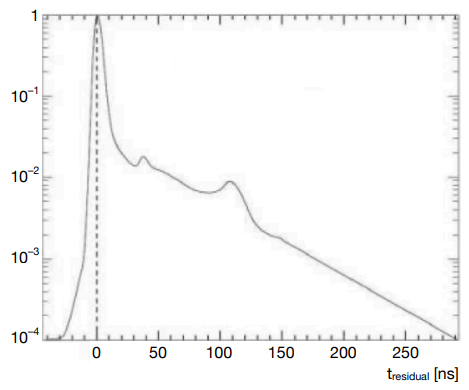
\includegraphics[scale=0.4]{Figures/bonsai_pdf_res.png}
\caption{Probability density of the timing residual P$(t-t_{\text {tof }}-t_{0})$, where $t_{0}$ use for the vertex reconstruction maximum likelihood fit. The peaks at 30ns and 100ns are caused by PMT after-pulsing. Figure from \cite[nakanopdf].}
    \label{bonsaivertexpdf}
\end{figure}

\begin{figure}
    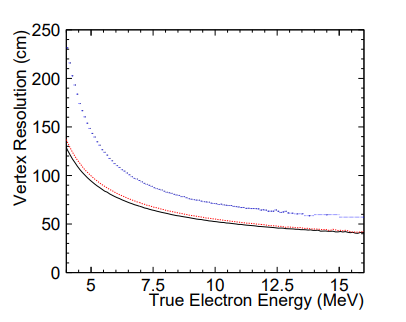
\includegraphics[scale=0.4]{Figures/bonsai_vertex_res.png}
\caption{The vertex resolution (the point at which 68\% of the events in the distance distribution between the actual and reconstructed vertex are contained) for the different SK phases. SK-I (Blue), SK-III (Red), SK-IV (Black).  Figure from \cite[nakanopdf].}
    \label{bonsaivertexres}
\end{figure}

\subsection{Direction Reconstruction}

Cherenkov light is emitted in a conical formation as electrons and positrons travel through water, with a Cherenkov angle of $\approx 42\degree$. BONSAI can reconstruct the direction of these particles by using this information along with the reconstructed vertex. This reconstruction occurs using a maximum likelihood function defined in Equation \ref{directionlikelihoodeq}.

\begin{equation}
    \mathcal{L}(\vec{d})=\sum_{i}^{N_{20}} \log (f(\cos\theta_{i}, E))\times\frac{\cos\theta_{i}}{a(\theta_{i})}
    \label{directionlikelihoodeq}
\end{equation}

$f(\cos\theta_{i},E)$ is the expected distribution of the angle between the vector of the direction $\vec{d}$ of the particle, and the observed Cherenkov photon from the position of the reconstructed vertex. The reason there is a spread in this energy distribution is because while the highest value of this distribution occurs at the cosine of the opening Cherenkov angle of $42\degree$, due to the particle travelling through the water being Coulomb scattered multiple times, there is a variation in the angle because of the varying particle energy. $N_{20}$ is the number of hits whose residual hit time is within 20ns of the time of the reconstructed event, which is used in order to reduce the amount dark noise and scattered photons contribute to the direction reconstruction calculation. The  variable $a(\theta_{i})$ is used in the second term in Equation \ref{directionlikelihoodeq}, and it is linked to the angle of incidence of the photon on the PMT $a(\theta_{i})$, and is a correction factor stemming from the acceptance of PMTs and therefore linked to the shape of the PMT and it's acrylic case. 





